\begin{figure*}[t]
	\centering
	\addtolength{\tabcolsep}{-4.5pt}
	\begin{tabular}{cccccccc}
		target & sample-1 & sample-2 & sample-3 & target & sample-1 & sample-2 & sample-3
		\\
		\begin{overpic}[width=\resultwidth]{fig6/2_leather_1/target.jpg}
			\imglabel{Leather-1}
		\end{overpic} &
		\includegraphics[width=\resultwidth]{fig6/2_leather_1/good1.jpg} &
		\includegraphics[width=\resultwidth]{fig6/2_leather_1/bad1.jpg} &
		\includegraphics[width=\resultwidth]{fig6/2_leather_1/bad2.jpg} &
		\begin{overpic}[width=\resultwidth]{fig6/3_plaster_2/target.jpg}
			\imglabel{Plaster-2}
		\end{overpic} &
		\includegraphics[width=\resultwidth]{fig6/3_plaster_2/good1.jpg} &
		\includegraphics[width=\resultwidth]{fig6/3_plaster_2/bad1.jpg} &
		\includegraphics[width=\resultwidth]{fig6/3_plaster_2/bad2.jpg}
		\\
		&
		\begin{overpic}[width=\resultwidth]{fig6/cell/cell_1.jpg}
			\put(0,0){\color{green}%
				\frame{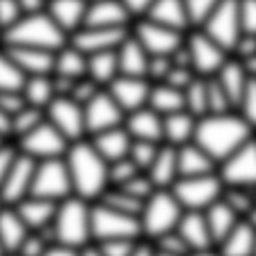
\includegraphics[width=0.4\resultwidth]{fig6/cell/cell_1_zoom.jpg}}}
		\end{overpic}
		&
		\begin{overpic}[width=\resultwidth]{fig6/cell/cell_2.jpg}
			\put(0,0){\color{green}%
				\frame{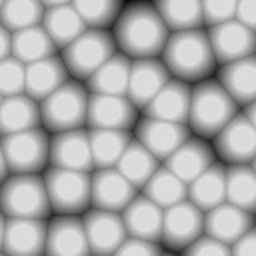
\includegraphics[width=0.4\resultwidth]{fig6/cell/cell_2_zoom.jpg}}}
		\end{overpic}
		&
		\begin{overpic}[width=\resultwidth]{fig6/cell/cell_3.jpg}
			\put(0,0){\color{green}%
				\frame{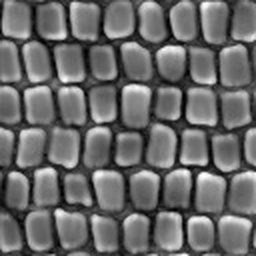
\includegraphics[width=0.4\resultwidth]{fig6/cell/cell_3_zoom.jpg}}}
		\end{overpic}
		&
		&
		\begin{overpic}[width=\resultwidth]{fig6/noise/noise_1.jpg}
			\put(0,0){\color{green}%
				\frame{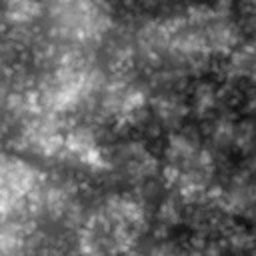
\includegraphics[width=0.4\resultwidth]{fig6/noise/noise_1_zoom.jpg}}}
		\end{overpic}
		&
		\begin{overpic}[width=\resultwidth]{fig6/noise/noise_2.jpg}
			\put(0,0){\color{green}%
				\frame{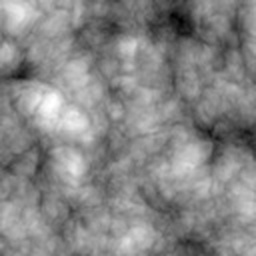
\includegraphics[width=0.4\resultwidth]{fig6/noise/noise_2_zoom.jpg}}}
		\end{overpic}
		&
		\begin{overpic}[width=\resultwidth]{fig6/noise/noise_3.jpg}
			\put(0,0){\color{green}%
				\frame{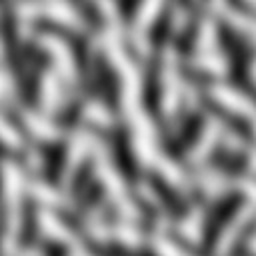
\includegraphics[width=0.4\resultwidth]{fig6/noise/noise_3_zoom.jpg}}}
		\end{overpic}
		%\\
		%\multicolumn{4}{c}{(b)}
	\end{tabular}
	\captionsetup{labelfont=bf,textfont=it}
	\caption{\label{fig:discrete}
		\textbf{MCMC sampling with discrete parameters.} In these examples, we illustrate the ability of our sampling to handle discrete parameters. In both examples, one noise inputs used in the procedural model can be switched between several different types of noise. Out of the thousands of sampled solutions, we pick three that have different settings of the discrete parameter where the (log) pdf values decrease from sample-1 to sample-3.
	}
\end{figure*}
